\chapter{Background}

\section{Introduction to NVM technology}
% 1. Short description of idea of NVM memory
% 2. Short description of benefits and drawbacks of using NVM memory
% 3. Differences between programming for volatile and non-volatile memory
\section{Introduction to Persistent Memory Development Kit}
\subsection{Overview}
% What is PMDK
\subsection{Libpmem library}
% Overview of low-level persistent memory support library
\subsection{Libpmemobj library}
% Overview of higher level library for C language providing transactions, memory allocation and concurrency support
\subsection{Libpmemobj++ library}
% Overview of C++ bindings for libpmemobj library

\section{Distributed hash table} % distributed hash table
  We want to create a distributed system that supports many nodes connection.
  The nodes can join and leave at any moment.
  With that system we will have the ability to distribute our hash table and support their read and write operations.

  Our main goal is to focus on high availability which is one of the most important component of CAP theorem nowadays.
  This means that every request gets a response on success or failure. 
  Achieving high availability in distributed system requires that the system have no downtimes and is operational all the time. Regardless of the state of any individual
  node in the system every client gets a response.

  We decided to follow the rules that Amazon stated in theirs solution: Amazon Dynamo \cite{AmazonDynamo}.
  Amazon is one of the largest e-commerce, cloud computing and artificial intelligence company.
  They have faced a challenge which was to serve millions of users concurrently.
  Their platform consist of tens of thousands of servers and network components located around the world.
  Because of that there is no possibility that every component works perfectly and never fail.
  Keeping that in mind they had to create a solution because even a small mistake could lead to a financial consequences and impact user customer trust.

  Amazon Dynamo is highly available key-value storage system that some core services of Amazon use to provide an "always-on" experience.
  For example Amazon Simple Storage Service also known as Amazon S3 is based on Dynamo.
  In Dynamo their key principles are:

\begin{itemize}
  \item \textit{Incremental scalability}:
    System should be able to scale out easily with minimal impact on operator. This means that connecting new node to a network
    wouldn't have a significant impact on performance of whole system. Because of that system can be easily scaled horizontally
    and would never reach a performance downgrade.
  \item \textit{Symmetry}:
    Every node in system is equal. This means that they have same set of responsibilities as its peers. There are no nodes that
    have extra commands nor responsibilities. This solution simplifies the process of maintaining system.
  \item \textit{Decentralisation}:
    This is an extension of symmetry. System design should favour decentralised peer-to-peer techniques over centralised control.
    Centralised control can result in outage and be a bottleneck of whole system. With that in mind decentralisation can lead to
    simpler, more scalable and more available system.
  \item \textit{Heterogeneity}:
    System infrastructure needs to be able to control work distribution. Amount of work given to a node should be proportional
    to the capabilities of the individual server. This is essential when adding new node with higher capacity without having to
    upgrade all hosts at once.
\end{itemize}

% - Consistent hashing
  To keep data synchronised between nodes we decided to use \textbf{consistent hashing}. This is because traditional hashing method
  during a change in number of array slots causes nearly all keys to be remapped. Which would have catastrophic impact for
  our system performance where different elements of hash table would have to move from one node to another.

  Consistent hashing is idea that does not depend directly on the number of nodes. Thanks to that when adding or removing
  node from a system the number of keys that need to remapped on average is $ K/n $, where $K$ is number of keys and $n$
  is number of nodes.

  Whole concept is based on abstract circle or hash ring which allows nodes and hash table objects to scale without affecting
  the overall system. We calculate hash value for each key and node and place them at hash ring. Minimal value correspond to
  angle 0 and the maximum possible value represent an angle of 360 degrees.
  Once we have both objects and nodes placed on the hash ring we can define a rule to associate which node is responsible for
  which object. Each object key belong to the node whose key is closest in counterclockwise direction (or clockwise depends on
  used convention). To find out what keys are node responsible for we need to locate node key on the circle and move in the
  ascending angle direction until we find another node. All objects encountered on this road belongs to this node.

  To be more consistent and distribute keys evenly among nodes, we can assign nodes not to one but to many places.
  The number of one node keys, known as \textit{weight}, depends on the situation and may be different for each node
  depending of node capabilities(\textit{heterogeneity}). Thanks to that solution we can easily remove or add nodes
  to a system and only $ K/n $ keys needs to be remapped.

\begin{figure}[h] %kn: wouldn't it be better to use [width=0.45\textwidth] instead of scale? 
        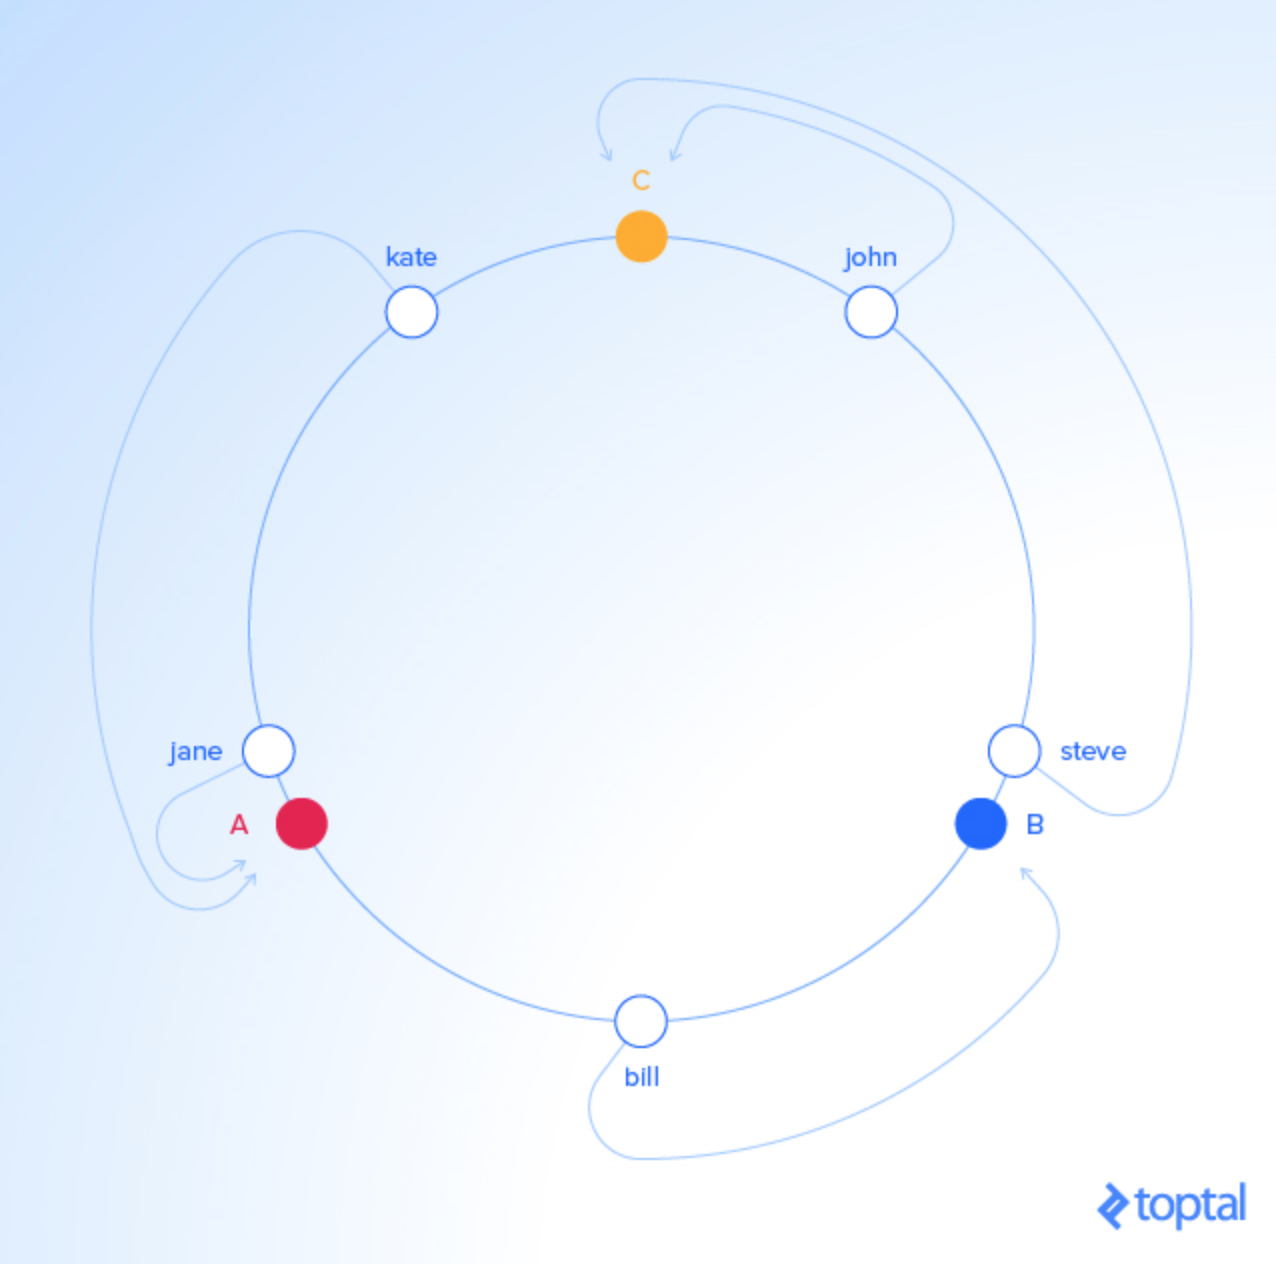
\includegraphics[scale=0.35]{thesis/figures/hashring.png}  
        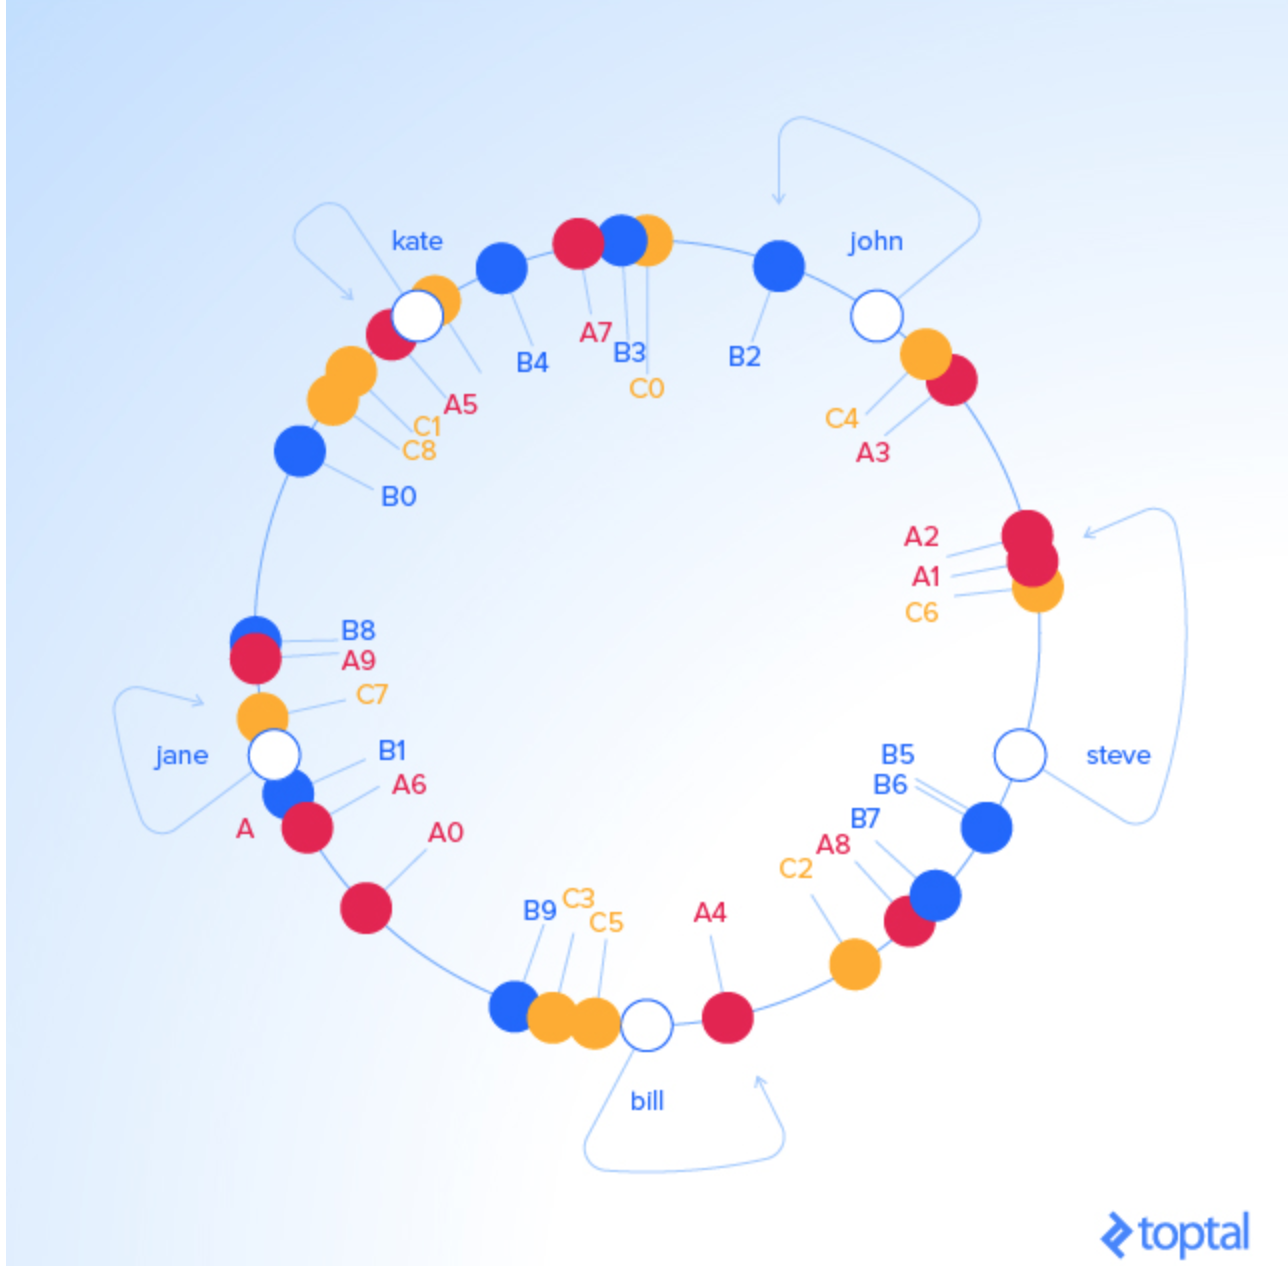
\includegraphics[scale=0.35]{thesis/figures/vnodes.png}
    \caption{Hash ring - names represents objects and letters represent nodes. 
            Left - nodes represented once at hashring.
            Right - nodes with many labels. \cite{ConsistentHashing}}
\end{figure}

%TODO Replication factor, seastar lib